\chapter{Efficient Incremental Search}
\label{chap:ibid}

Solving the dynamic single-pair shortest path (SPSP) problem.
AKA two-terminal shortest-path problem.

Bidirectional approach:
Partially solve a single-source shortest-path (SSSP) problem
and the complementary single-destination shortest-path problem (SDSP).

Motivate this with LazySP.
What if your heuristic is not that great?

Combine bidirectional search,
heuristic-guided search,
and incremental search.

Solve the Bellman-Ford equations in the correct order.

This is a relatively straightforward integration of incremental search
(DynamicSWSF-FP \citep{ramalingam1996})
and bidirectional Dijkstra's search \citep{goldberg2005spexternalmemory}.
The most subtle part of the algorthm is getting the termination
condition right.
The benefit of bidirectional search for an problem that is
uninformed by a heuristic
is that it tends to explore a smaller subset of the graph
(view bubbles).
We have found that some problems with weak heuristics,
it outperforms LPA*.
See some plots below.

\begin{table}
\centering
\begin{tabular}{ccc}
   \toprule
   & Unidirectional & Bidirectional \\
   \midrule
   \addlinespace[0.2em]
   Complete
      & Dijkstra \citep{dijkstra1959anote}
      & Bidirectional Dijkstra \citep{luby1989bidijk} \\
   \addlinespace[-0.2em]
   \emph{(Heuristic)}
      & \emph{A* \citep{hart1968astar}}
      & \emph{Bidirectional A* \citep{ikeda1994betterroutes}} \\
   \addlinespace[0.3em]
   Incremental
      & DynamicSWSF-FP \citep{ramalingam1996}
      & \multirow{2}{*}{IBID}  \\
   \addlinespace[-0.2em]
   \emph{(Heuristic)}
      & \emph{Lifelong Planning A* \citep{koenig2004lpastar}}
      & \\
   \addlinespace[0.2em]
   \bottomrule
\end{tabular}
\caption{A table.}
\end{table}

We are not interested in domains that are chiefly memory-constrained,
so no need to consider iterative-deepening approaches,
including bidirectional variants as proposed by
Kaindl and Kainz, ``Bidirectional Heuristic Search Reconsidered,''
Journal of AI Research 1997.

\section{Prior Work}

The \emph{shortest path problem} on graphs has been extensively
studied over the past six decades.
Consider a directed graph $G = (V,E)$ and accompanying edge weight
function $w : E \rightarrow \mathbb{R}$,
with the length of a path equal to the sum of the weights of its
constituent edges.
I include here a brief survey of algorithmic work on the
\emph{single-pair} (a.k.a. point-to-point) problem,
where a path of minimal length is sought
between particular source and target vertices
$s,t \in V$.
I also consider only graphs without negative-length cycles.

\subsection{Pathfinding via the Source Distance Function}

The pioneering pathfinding algorithms of the late 1950s address
the \emph{single-source} problem,
where shortest paths are calculated from $s$ to all vertices on
the graph.
They proceed by calculating the \emph{distance function}
$d_s : V \rightarrow \mathbb{R}$,
which is characterized by
\begin{equation}
   d_s(s) = 0
   \quad\mbox{and}\quad
   \forall v \neq s,\;
   d_s(v) = \min_{u \in \mbox{\scriptsize Pred}(v)} d_s(u) + w(u,v).
   \label{eqn:distance-function}
\end{equation}
The distance function is akin to the \emph{value function}
in more general decision problems addressed by dynamic programming,
and (\ref{eqn:distance-function}) is the Bellman equation
\citep{bellman1958routing}.
This characterization also follows implicitly from early results for
the all-pairs problem
\citep{shimbel1955communicationnets, beckmann1955transportation}.
A shortest path to a target $t$ can be generated trivially
by walking backwards to $s$ guided by the function $d_s$.

Algorithms for computing $d_s$ rely on the concept of
\emph{relaxation}
as described by Ford \citep{ford1955networkflowtheory}.
The function $d_s$
is initialized to the upper bound $\infty$ for $v \neq s$,
and edges $(u,v)$ for which $d_s(v) > d_s(u) + w(u,v)$,
thereby violating (\ref{eqn:distance-function}),
are relaxed by updating $d_s(v)$
with the reduced value $d_s(u) + w(u,v)$.
The well-known Bellman-Ford method
\citep{shimbel1955communicationnets, bellman1958routing,
moore1959spmaze}
iterates through all edges repeatedly until convergence
(at most $|V|$ repetitions are sufficient).

Soon afterwards,
several researchers
identified \citep{leyzorek1957modeltechniques, dijkstra1959anote}
an efficient ordering of edge relaxations
if $w$ is non-negative.
Dijkstra's algorithm relaxes edges $(u,v)$
in increasing order of $d_s(u)$.
In does this by initially marking all vertices as {\sc Open},
and at each iteration moving to {\sc Closed}
the vertex $u$ minimizing $d_s$
and relaxing all outgoing edges $(u,v)$ from $u$.
It is guaranteed to consider each vertex
(and therefore relax each edge) at most once.

\subsection{Bidirectional Search}

The single-pair problem can therefore be solved
via Dijkstra's algorithm
by (partially) computing the source distance $d_s$ until it
includes the target vertex.
However,
it was conjectured that a path might be found more efficiently
by simultaneously calculating the complementary
target distance function $d_t$
until the domains of the two functions ``overlap.''
The first mention of such a bi-directional algorithm
was proposed by Dantzig \citep{dantzig1963linearprogramming},
and the first precisely described algorithm was presented by
Nicholson \citep{nicholson1966shortest}.
Implementation of a sound and efficient algorithm
turns on two important questions:
(a) how to balance the two directions of the search,
and (b) when and how to terminate with a shortest path.

A correct termination condition is surprisingly subtle,%
\marginnote{There were early incorrect attempts at a sound
termination condition
\citep{berge1965programminggamestransportation}.}
with several correct variations proposed
\citep{nicholson1966shortest, dreyfus1969appraisalsp,
pohl1969bidirectional, goldberg2005spexternalmemory}.
The difficulty stems from the fact that the first vertex to be
{\sc Closed} by the searches in both directions
need not lie on the shortest path.

The general bidirectional algorithm also leaves open the strategy
used to balance the progression of the two search directions.
Options based on alternating \citep{dantzig1963linearprogramming},
or selecting the direction with the smaller {\sc Open} distance
\citep{nicholson1966shortest}
or {\sc Open} (and finite) set cardinality
\citep{pohl1969bidirectional}
were proposed.
It was further shown that selecting only from the source direction
reproduces Dijkstra's algorithm.

\subsection{Heuristic Search}

Heuristic methods such as the Graph Traverser
\citep{doran1966graphtraverser} were originally
applied to pathfinding problems in order to find non-optimal
solutions more economically.
These unidirectional methods proceed similarly to Dijkstra's algorithm,
but instead of prioritizing {\sc Open} vertices
based on their source distance $d_s$,
they use a target-directed heuristic function $h_t$.
Hart, Nilsson, and Raphael \citep{hart1968astar} discovered that
these approaches can be combined ($d_s + h_t$) to yield
an admissible algorithm (A*) for the shortest-path problem,
as long as $h_t$ meets certain conditions.

Attempts to provide a bidirectional algorithm which incorporates
heuristics generally take one of three approaches.
\cdnote{I need to deep-dive here to write this correctly.}

First,
front-to-front methods
could evaluate the heuristic between all pairs in the two
{\sc Open} sets.
Expensive.

Second,
perform two heuristic-informed searches,
and account for the connection problem via a complex
termination condition.
Not necessarily efficient.
(Pohl cites Berge?)
Missile analogy.

Third,
waste (same heuristic function).

Concept of waste \citep{pohl1969bidirectional}.
I think this subsumes A*.

Talk about the 94 paper \citep{ikeda1994betterroutes}
expressing A* as a search on
the waste graph.

As a potential function.
Also Goldberg \citep{goldberg2005spexternalmemory}.

To integrate: \citep{dechter1984bfsastaropt}.

\subsection{Incremental Search}

This stuff is more modern (1996, 2004).

DynamicSWSF-FP \citep{ramalingam1996}.

Revisit Bellman equation.

Apply waste to incremental search to get
incremental heuristic search.

\subsection{Incremental Heuristic Search}

Lifelong Planning A* \citep{koenig2004lpastar}.

\section{Termination Conditions}

What happens upon an encounter between the forward and reverse searches?
Goldberg \citep{goldberg2005spexternalmemory}
discusses the correct termination condition for the 
Bidirectional Dijkstra algorithm.

\section{Prioritizing Directions}

So, we can conduct expansions from the queues for either direction.
How should we proceed?
We do so via what (Pohl 1971) called a ``cardinality criterion''.

\section{The Algorithm}

The main outline of IBiD is given in Algorithm~\ref{alg:ibid}.
IBiD conducts two independent DynamicSWSF-FP searches
(Algorithm~\ref{alg:ibid-two-dynamicswsffps}).

\begin{algorithm}[t]
   \caption{IBiD Outline}
   \label{alg:ibid}
   \begin{algorithmic}[1]
      \Procedure {Main} {\,}
         \State $\mbox{\sc InitializeSource}(); \; \mbox{\sc InitializeTarget}()$
         \State $Q_c \gets \emptyset$
            \Comment $\mbox{ key for } (u,v): d_s(u) + w(u,v) + d_t(v)$
         \Loop
            \While {not $\mbox{\sc TerminationCondition}()$}
               \If {$Q_s.\mbox{TopKey} < Q_t.\mbox{TopKey}$}
                     \Comment prioritize arbitrarily
                  \State $\mbox{\sc ProcessSourceQueue}(u)$
               \Else
                  \State $\mbox{\sc ProcessTargetQueue}(u)$
               \EndIf
               \State Ensure $(u,v) \in Q_c$ iff
                  $u \neq Q_s$, $v \neq Q_t$, key $\neq \infty$
            \EndWhile
            \State $(u_c,v_c) \gets Q_c.\mbox{Top}$
            \State $\pi \gets
               ( \mbox{walk } d_s \mbox{ from } u_c \mbox{ to } s )
               \cup
               ( \mbox{walk } d_t \mbox{ from } v_c \mbox{ to } t )$
            \State wait for edges $(u,v) \in E_{\ms{delta}}$ with changed weights $w(u,v)$
            \State $\mbox{\sc NotifyWeightChanges}(E_{\ms{delta}})$
         \EndLoop
      \EndProcedure
      \Function {TerminationCondition} {\,}
         \State $(u_c,v_c) \gets Q_c.\mbox{TopKey}$
            \Comment return False if $Q_c$ empty
         \If {$Q_s.\mbox{TopKey} + Q_t.\mbox{TopKey} < d_s(u_c) + w(u_c,v_c) + d_t(v_c)$}
            \State \Return False
         \EndIf
         \If {$Q_s.\mbox{TopKey} < d_s(u_c)$
               \mbox{\bf or} $Q_t.\mbox{TopKey} < d_t(v_c)$}
            \State \Return False
         \EndIf
         \State \Return True
      \EndFunction
      \Procedure {NotifyWeightChanges} {$E_{\ms{delta}}$}
         \ForAll {$(u,v) \in E_{\ms{delta}}$}
            \State $\mbox{\sc UpdateSourceDistance}(v)$
            \State $\mbox{\sc UpdateTargetDistance}(u)$
         \EndFor
         \State Ensure $(u,v) \in Q_c$ iff
            $u \neq Q_s$, $v \neq Q_t$, key $\neq \infty$
      \EndProcedure
   \end{algorithmic}
\end{algorithm}

{\floatevery{algorithm}{\setlength\hsize{16.85cm}}
\begin{algorithm}[t]
   \caption{As a bidirectional algorithm,
      IBiD conducts two independent DynamicSWSF-FP searches,
      one computing distance from the source vertex,
      and the other computing distance to the target vertex.}
   \label{alg:ibid-two-dynamicswsffps}
   \begin{minipage}[t]{8.2cm}
      \begin{algorithmic}[1]
         \Procedure {InitializeSource} {\,\!}
            \ForAll {$v \in V$}
               \State $d_s(v) \gets \infty; \;\; r_s(v) \gets \infty$
            \EndFor
            \State $r_s(s) \gets 0$
            \State $Q_s \gets \{ s \}$
               \Comment $\mbox{ key for } v: \min\big(r_s(v),d_s(v)\big)$
            \State $\mbox{\sc ProcessSourceQueue}()$
         \EndProcedure
         \Procedure {UpdateSourceDistance} {$v$}
            \If {$v \neq s$}
               \State $r_s(v) \gets \displaystyle\min_{u \in \mbox{\scriptsize Pred}(v)}
                  \big( d_s(u) + w(u,v) \big)$
            \EndIf
            \State Ensure $v \in Q_s$ iff $d_s(v) \neq r_s(v)$
         \EndProcedure
         \Procedure {ProcessSourceQueue} {\,\!}
            \State $u \gets Q_s.\mbox{Pop}$
            \If {$r_s(u) < d_s(u)$}
                  \Comment over-consistent
               \State $d_s(u) \gets r_s(u)$
               \ForAll {$v \in \mbox{Succ}(u)$}
                  \State $\mbox{\sc UpdateSourceDistance}(v)$
               \EndFor
            \Else
                  \Comment under-consistent
               \State $d_s(u) \gets \infty$
               \ForAll {$v \in \mbox{Succ}(u) \cup u$}
                  \State $\mbox{\sc UpdateSourceDistance}(v)$
               \EndFor
            \EndIf
         \EndProcedure
         \algstore{ibid-two-dynamicswsffps}
      \end{algorithmic}
   \end{minipage}
   \quad
   \begin{minipage}[t]{8.2cm}
      \begin{algorithmic}[1]
         \algrestore{ibid-two-dynamicswsffps}
         \Procedure {InitializeTarget} {\,\!}
            \ForAll {$v \in V$}
               \State $d_t(v) \gets \infty; \;\; r_t(v) \gets \infty$
            \EndFor
            \State $r_t(t) \gets 0$
            \State $Q_t \gets \{ t \}$
               \Comment $\mbox{ key for } v: \min\big(r_t(v),d_t(v)\big)$
            \State $\mbox{\sc ProcessTargetQueue}()$
         \EndProcedure
         \Procedure {UpdateTargetDistance} {$u$}
            \If {$u \neq t$}
               \State $r_t(u) \gets \displaystyle\min_{v \in \mbox{\scriptsize Succ}(u)}
                  \big( w(u,v) + d_t(v) \big)$
            \EndIf
            \State Ensure $u \in Q_t$ iff $d_t(u) \neq r_t(u)$
         \EndProcedure
         \Procedure {ProcessTargetQueue} {\,\!}
            \State $v \gets Q_t.\mbox{Pop}$
            \If {$r_t(v) < d_t(v)$}
                  \Comment over-consistent
               \State $d_t(v) \gets r_t(v)$
               \ForAll {$u \in \mbox{Pred}(v)$}
                  \State $\mbox{\sc UpdateTargetDistance}(u)$
               \EndFor
            \Else
                  \Comment under-consistent
               \State $d_t(v) \gets \infty$
               \ForAll {$u \in \mbox{Pred}(v) \cup v$}
                  \State $\mbox{\sc UpdateTargetDistance}(u)$
               \EndFor
            \EndIf
         \EndProcedure
      \end{algorithmic}
   \end{minipage}
\end{algorithm}
} % floatevery width adjustment

\section{Examples}

See Figure~\ref{fig:incbi-lpastar-fig1-heurchange}
and Figure~\ref{fig:incbi-lpastar-fig1}.

\begin{figure}
   \centering%
   
   \includegraphics{build/incbi-lpastar-fig1/lpastar-heurnone-original}%
   \;\;%
   \includegraphics{build/incbi-lpastar-fig1/incbi-heurnone-original}%
   
   \vspace{0.2cm}
   
   \includegraphics{build/incbi-lpastar-fig1/lpastar-heurhalf-original}%
   \;\;%
   \includegraphics{build/incbi-lpastar-fig1/incbi-heurhalf-original}%
   
   \vspace{0.2cm}
   
   \includegraphics{build/incbi-lpastar-fig1/lpastar-heurfull-original}%
   \;\;%
   \includegraphics{build/incbi-lpastar-fig1/incbi-heurfull-original}%
   
   \caption{Illustration of behavior of IBiD on a single
      (non-incremental) shortest path problem.
      At left, IBiD uses the unidirectional start-side expansion
      strategy.
      At right, IBiD uses the bidirectional distance-balanaced
      expansion strategy.
      Start and goal heuristic functions are available;
      the unidirectional search uses a potential function based
      on the goal heuristic,
      and the bidirectional search a potential function using
      the average heuristic.
      IBiD is run with three different potential function weights:
      0.0 (top), 0.5 (middle), and 1.0 (bottom).
      IBiD therefore preforms equivalently to
      Dijkstra's algorithm (top-left),
      Bidirectional Dijkstra's (top-right),
      A* (bottom-left),
      and Bidirectional A* (bottom-right).}
   \label{fig:incbi-lpastar-fig1-heurchange}
\end{figure}

\begin{figure}
   \centering%
   
   \includegraphics{build/incbi-lpastar-fig1/lpastar-heurfull-original}%
   \;\;%
   \includegraphics{build/incbi-lpastar-fig1/lpastar-heurfull-changed}%
   
   \vspace{0.2cm}
   
   \includegraphics{build/incbi-lpastar-fig1/incbi-heurfull-original}%
   \;\;%
   \includegraphics{build/incbi-lpastar-fig1/incbi-heurfull-changed}%
   
   \caption{IBiD with only source-side expansions and a goal-side
      heuristic (top) proceeds identically to Lifelong Planning A*,
      performing 37 expansions on the original world (left)
      followed by 18 expansions over 14 vertices on the chanced
      world (right).
      IBiD with distance-balanced expansions and an average
      potential (bottom)
      performs 30 expansions on the original world
      followed by 18 expansions over 15 vertices on the changed
      world.}
   \label{fig:incbi-lpastar-fig1}
\end{figure}

\begin{figure*}
   \centering%
   
   \begin{tabular}{ccc}
      \specialcell{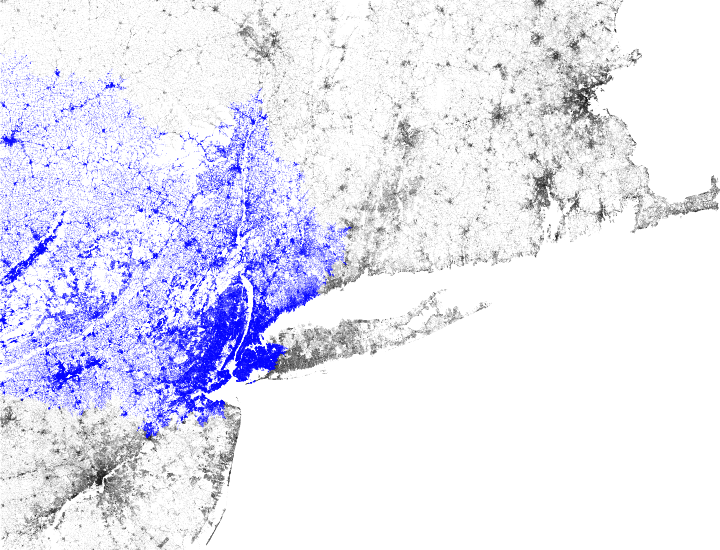
\includegraphics[width=5cm]{figs/incbi-road-ne/pgoalnone-balfwd.png}\\556,209 expansions}
      &
      \specialcell{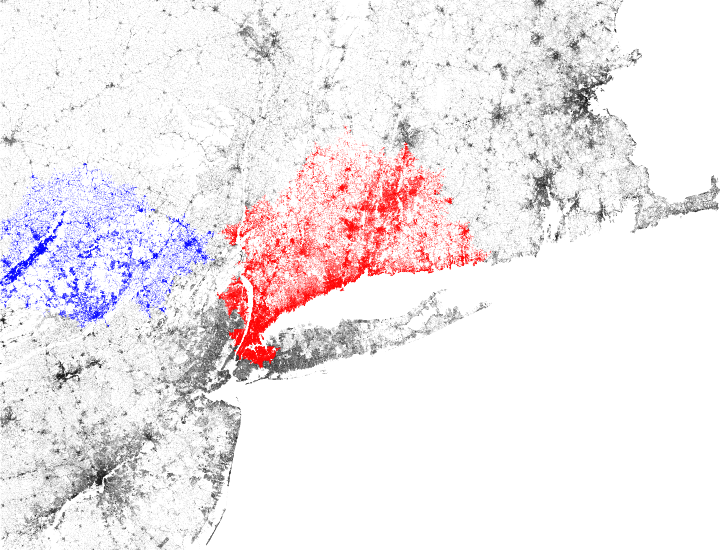
\includegraphics[width=5cm]{figs/incbi-road-ne/pavgnone-baldist.png}\\319,938 expansions}
      &
      \specialcell{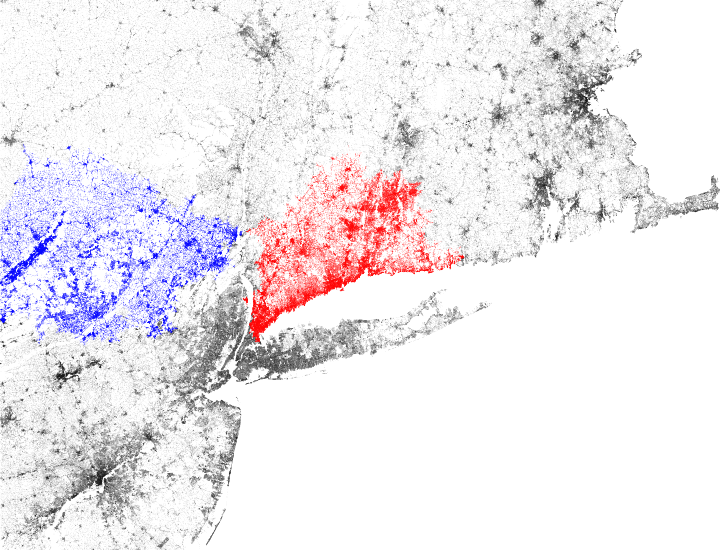
\includegraphics[width=5cm]{figs/incbi-road-ne/pavgnone-balcard.png}\\281,413 expansions}
      \vspace{0.3cm}
      \\
      \specialcell{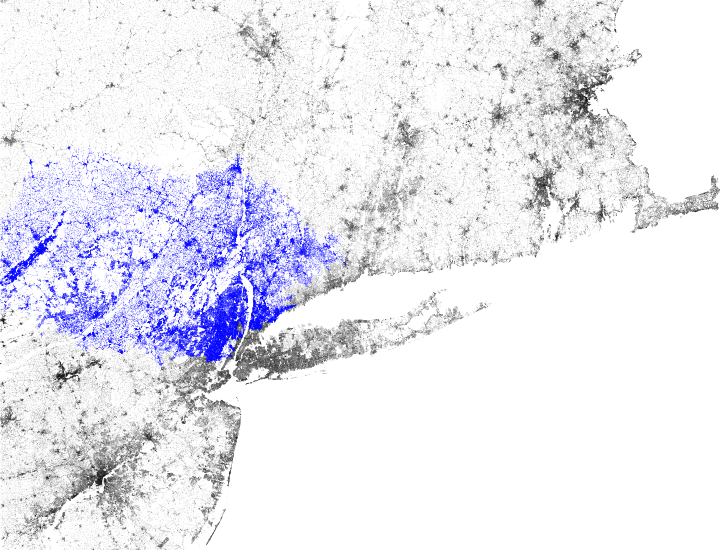
\includegraphics[width=5cm]{figs/incbi-road-ne/pgoalhalf-balfwd.png}\\297,414 expansions}
      &
      \specialcell{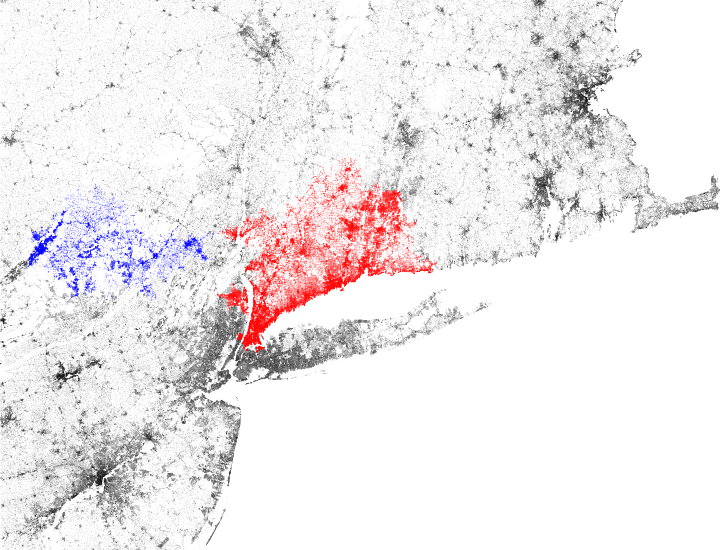
\includegraphics[width=5cm]{figs/incbi-road-ne/pavghalf-baldist.png}\\206,625 expansions}
      &
      \specialcell{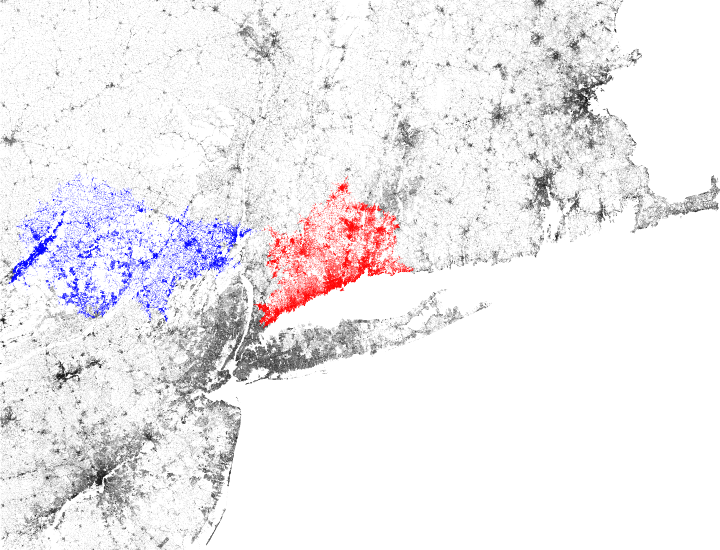
\includegraphics[width=5cm]{figs/incbi-road-ne/pavghalf-balcard.png}\\178,929 expansions}
      \vspace{0.3cm}
      \\
      \specialcell{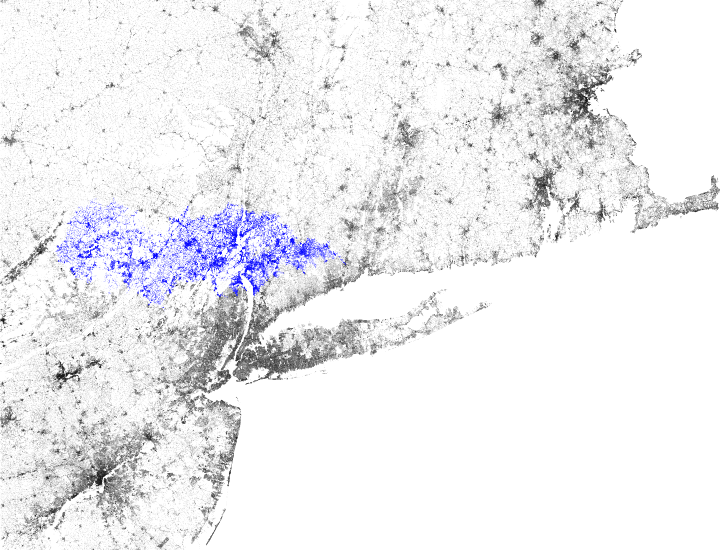
\includegraphics[width=5cm]{figs/incbi-road-ne/pgoalfull-balfwd.png}\\82,915 expansions}
      &
      \specialcell{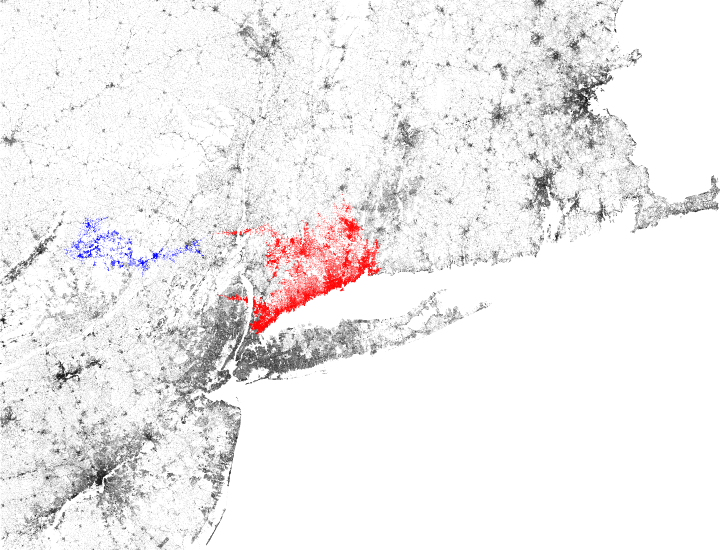
\includegraphics[width=5cm]{figs/incbi-road-ne/pavgfull-baldist.png}\\95,759 expansions}
      &
      \specialcell{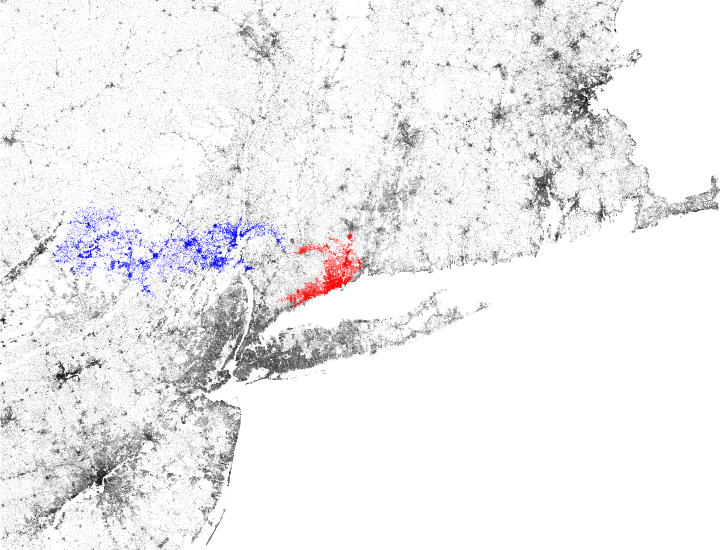
\includegraphics[width=5cm]{figs/incbi-road-ne/pavgfull-balcard.png}\\69,218 expansions}
      \vspace{0.5cm}
   \end{tabular}
   
   \caption{Comparison between various heuristic strengths and
      balancing strageties on a single-pair road network problem.
      A path with shortest transit time is sought.
      The heuristic strength varies from no heuristic (top)
      to a full-strength heuristic (bottom).
      At left, a foward-only balancer is used, so that the
      top-left is equivalent to Dijkstra's algorithm,
      and the bottom-left is equivalent to A*.
      The middle column uses a balanced distance strategy.
      The right column uses a balanced cardinality strategy.}
   \label{fig:incbi-road-ne}
\end{figure*}
